\chapter{Control}\label{ch:control}

\title{Control}

This chapter will extend what was derived previously from the mathematical model, analyse the behaviour of the modelled system through simulations and address the cruise control and cartesian stabilization control problems, later implemented on a physical system. 

\section{Cruise Control}

In this section we will look closer at the cruise control problem and the subsequent controller. Cruise control is essential for the robot since it ensures, that it keeps following a straight line and a certain angle with respect to the global co-ordinate axis. Since, the motor model derived in chapter \ref{ch:modeling}is linear, we can apply classical control techniques in order to design the controller.

In the cruise control we want to manipulate the velocity and the angular speed of the robot. In order to do, each of the wheels angular speed namely $\omega_{r}$ and $\omega_{l}$, must be controlled 

{\color{red} HERE GOES A FIGURE WHAT SHOWS ROBOT IN GLOBAL CO-ORDINATES}

In the following figure you can see the closed loop block diagram for the motor speed control. The plant in this diagram is the same motor model as we looked in the previous chapter.

\begin{figure}[H]
	\centering
 	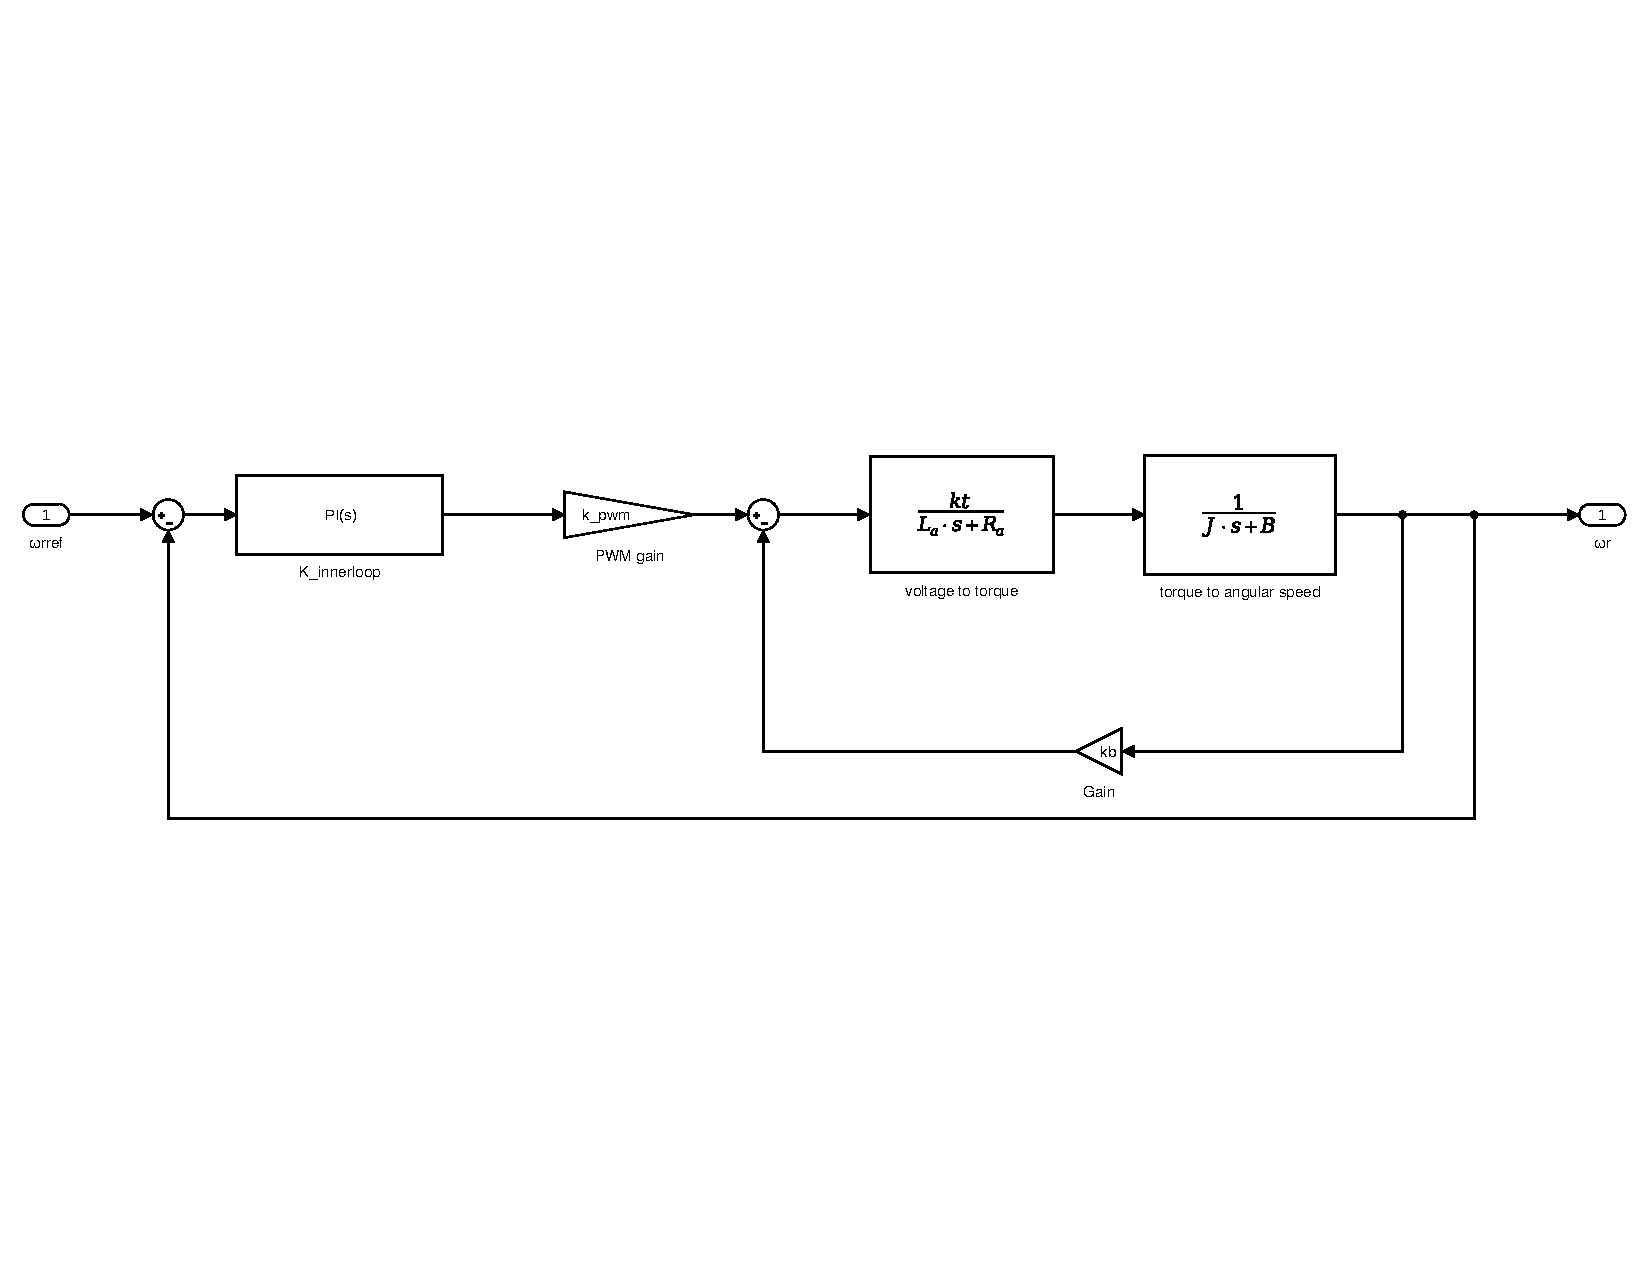
\includegraphics[width=1\textwidth]{figures/motorspeedcontrolclosedloop.pdf}
	\caption{Motor speed control} 
 	\label{fig:speedcontrol} 
\end{figure}

The block diagram consists of the motor plant,$K_{innerloop}$ the PI controller that we have designed to meet our desires. $P_{innerloop}$ is the motor model and the PWM gain $k_{pwm}$ put together. As a result we get the following equation:

\begin{equation}
P_{innerloop}=\frac{k.k_{pwm}}{k^2+(sL_{a}+R_{a})(sJ+B)}=\frac{4200}{(s+0.94)(s+4421)}
\end{equation}
\todo{modify}

Next we will look at the $K_{innerloop}$. This is the PI controller required to meet some specification. 

\begin{equation}
K_{innerloop}=\frac{g(s+z)}{s}*[\frac{100}{s+100}]^2
\end{equation} 

Following we can see that the open loop transfer function is given by the following equation:

\begin{equation}
G_{innerloop}=P_{innerloop}*K_{innerloop}
\end{equation}

Subsequently, the closed loop transfer is as follows:

\begin{equation}
H_{innerloop}=\frac{G_{innerloop}}{G_{innerloop}+1}
\end{equation}

For the simulations we used three different values on the g and z. For the first simulation we used z=1 and g=7. In the second simulation we used z=5 and g=5. for the final one we used z=10 and g=6.

The bode plots of the simulation can be seen below.

\begin{figure}{H}
\centering
 	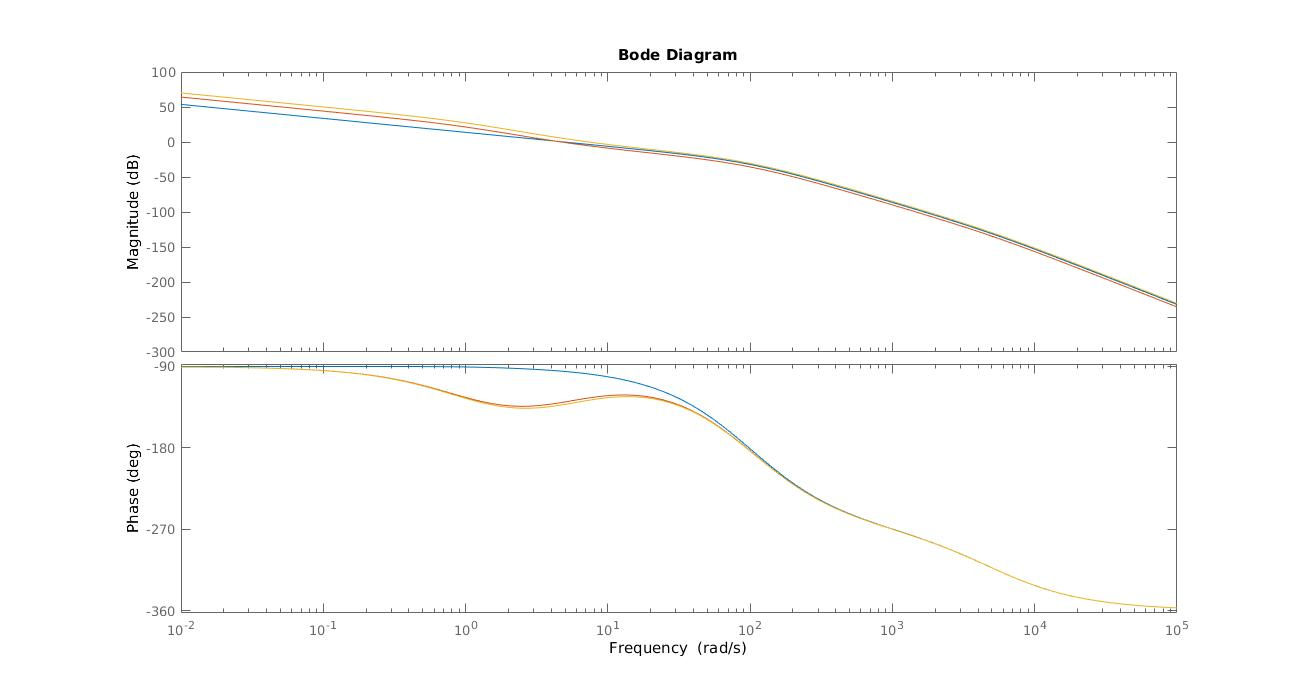
\includegraphics[width=1\textwidth]{figures/Ginnerbode.jpg}
	
	
	\caption{$G_{innerloop}$ bode plot} 
 	\label{fig:ginnerloopbode} 
\end{figure}

\begin{figure}{H}
\centering
 	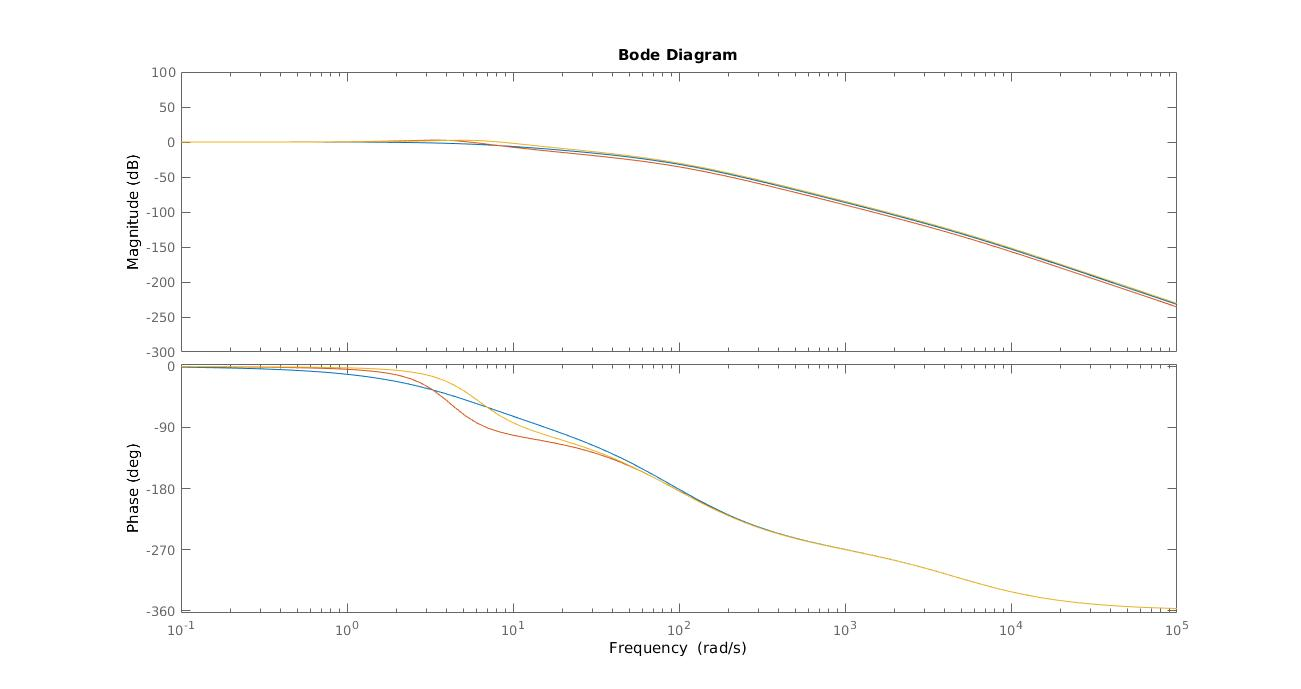
\includegraphics[width=1\textwidth]{figures/Hinnerbode.jpg}
	
	
	\caption{$H_{innerloop}$ bode plot} 
 	\label{fig:hinnerloopbode} 
\end{figure}

From the next figure you can see the step response of the three different controller configurations.

\begin{figure}{H}
\centering
 	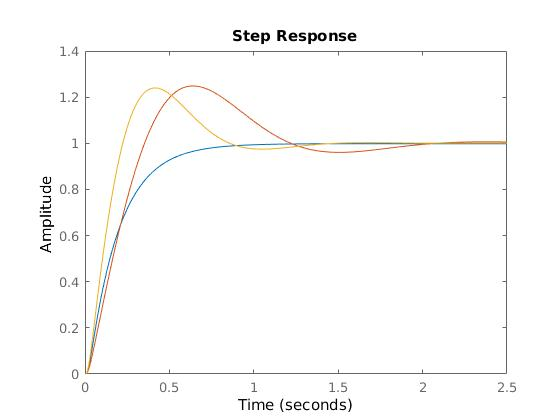
\includegraphics[width=1\textwidth]{figures/stepresponse.jpg}
	
	
	\caption{Step response} 
 	\label{fig:stepresponse} 
\end{figure}

\subsection{Angle control}

In order to develop the complete architecture of the cruise control we must first perform manipulation on the equations describing the differential drive configuration. By inverting  the matrix describing the relations between the individual wheel velocities and the robot input velocities  look how can we obtain $\omega_{rref}$ and $\omega_{lref}$ from $\omega$ and $v$ by:

\begin{equation} \label{eq66}
 \begin{pmatrix} 
 \omega_{rref} \\ 
 \omega_{lref} \\
 \end{pmatrix} 
 =
 \begin{pmatrix}  
 \frac{1}{r}   & \frac{l}{2r} \\ 
 \frac{1}{r} & \frac{-l}{2r} \\ 
 \end{pmatrix}
 \begin{pmatrix} 
 v_{ref} \\ 
 \omega_{ref}
 \end{pmatrix} 
 \end{equation} 

\begin{equation} \label{eq67}
M^{-1}
=
\begin{pmatrix}  
 \frac{1}{r}   & \frac{l}{2r} \\ 
 \frac{1}{r} & \frac{-l}{2r} \\ 
 \end{pmatrix} 
\end{equation}

The whole cruise control layout can be seen in figure~\ref{fig:cruisecontrol}.

\begin{figure}{H}
\centering
 	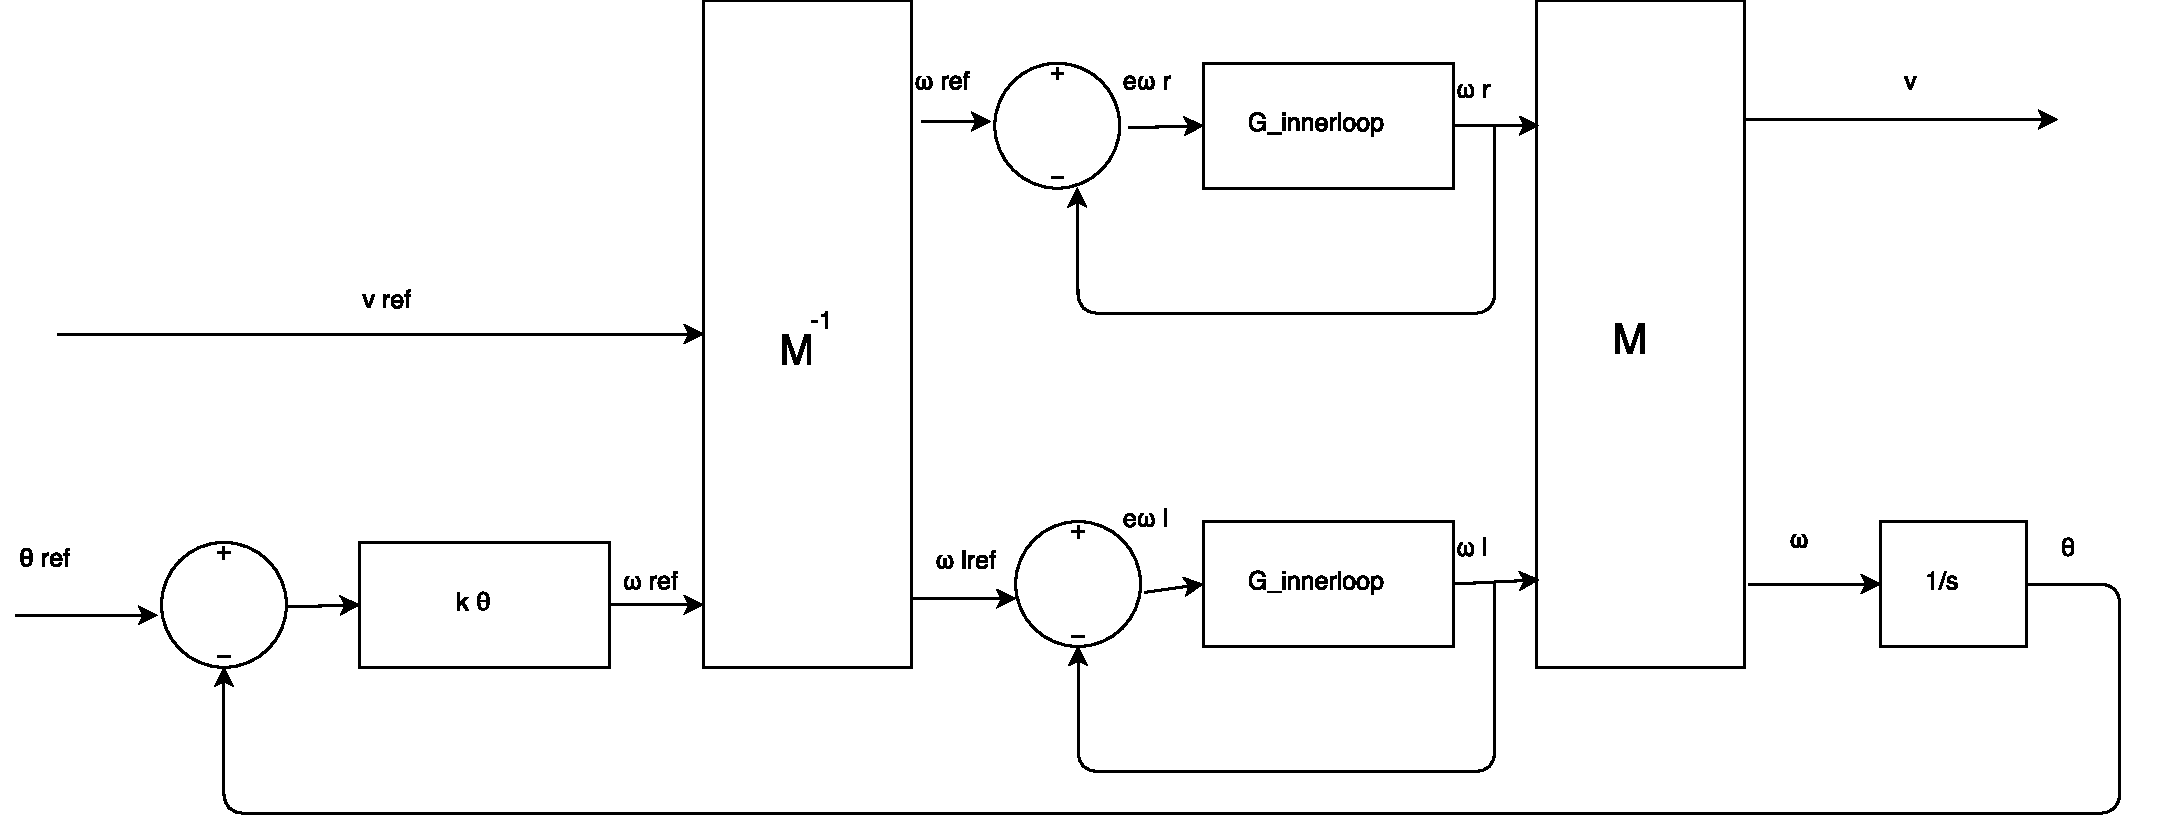
\includegraphics[width=1\textwidth]{figures/cruisecontrol.pdf}
	\caption{Cruise control full architecture} 
 	\label{fig:cruisecontrol} 
\end{figure}

In equations \ref{eq66} and \ref{eq67} we have $\omega_{rref}$ and $\omega_{lref}$,the separate wheels angular speeds that are fed to the motor subsystem. $v_{ref}$ is the desired linear speed of the robot and $\omega_{ref}$ is the desired angular speed of the whole robot. $r$ is the radius of the wheels and $l$ is the length between the wheels.

Further analysis on the equations leads to the identification of the transfer functions from the referenced linear speed($v_{ref}$) to the linear speed ($v$). Similarly, we can identify the transfer function from $\omega_{ref}$ to $\omega$. This tells us that the $v_{ref}$ to $v$ and $\omega_{ref}$ to $\omega$ time and frequency responses are the same as the motor speed responses. Using that knowledge we combine the equations in \ref{eq68} and \ref{eq69}

\begin{equation} \label{eq68}
 \begin{pmatrix} 
 v(s) \\ 
 \omega(s) \\
 \end{pmatrix} 
 =
 M^{-1}
 \begin{pmatrix}  
 H_{innerloop}(s)   & 0 \\ 
 0 & H_{innerloop}(s) \\ 
 \end{pmatrix}
 M
 \begin{pmatrix} 
 v_{ref}(s) \\ 
 \omega_{ref}(s)
 \end{pmatrix} 
 \end{equation}

\begin{equation} \label{eq69}
\frac{v(s)}{v_{ref}(s)}
=
\frac{\omega(s)}{\omega_{ref}(s)}
=
H_{innerloop}(s)
\end{equation}

In equations \ref{eq68} and \ref{eq69} the $v_{ref}$ is the linear velocity command and the $\omega_{ref}$ is the angular speed command for the robot.

Next part of the cruise control is to make the robot follow $\theta_{red}$ the commanded angle. Examining the figure \ref{fig:cruisecontrol} we can see that the plant for the angle control is given by

\begin{equation} \label{eq70}
P_{\Theta}
=
\frac{H_{innerloop}}{s}
=
\frac{24570}{(s+4995)(s+4.957)s}
\end{equation}

For simplicity, we will simplify the angle control block diagram to what can be observed in figure \ref{fig:anglecontrol}

\begin{figure}{H}
\centering
 	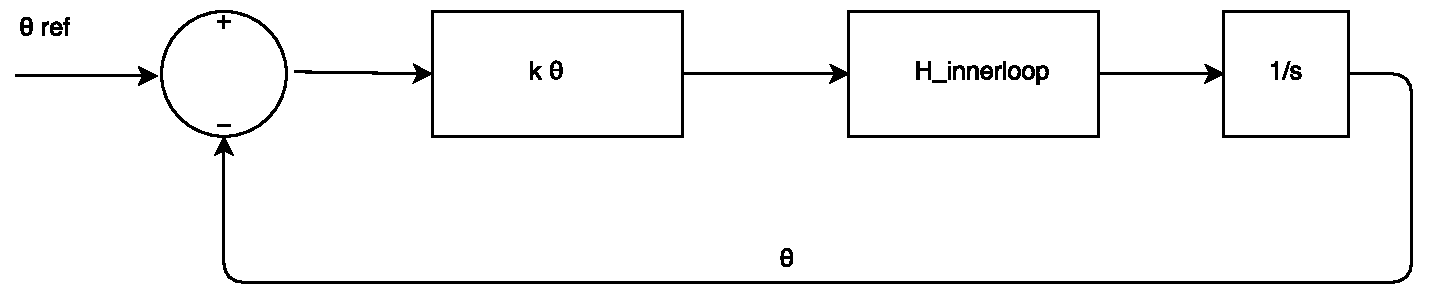
\includegraphics[width=1\textwidth]{figures/cropanglecontrol.pdf}
	
	
	\caption{$\Theta$ control} 
 	\label{fig:anglecontrol} 
\end{figure}

For controlling the $\Theta$ we will use a proportsional controller. The form of the controller $k_{\theta}$ is shown in the equation \ref{eq71}.

\begin{equation} \label{eq71}
k_{\theta}
=
g
\end{equation}

Furthermore we can obtain the transfer function for the open loop loop ($G_{\theta}$) given by:

\begin{equation} \label{eq72}
G_{\theta}
=
P_{\theta}k_{\theta}
\end{equation}

From here we can get the closed loop loop transfer function, which we will call $H_{\theta}$, as shown in the equation \ref{eq73}

\begin{equation} \label{eq73}
H_{\theta}
=
\frac{G_{\theta}}{G_{\theta}+1}
\end{equation}

Figure \ref{fig:gthetabode} shows the bode plot of the $G_{\theta}$, figure \ref{fig:hthetabode} the bode plot of the $H_{\theta}$, and figure /ref{fig:thetastep} the step response for the different controllers.

\begin{figure} 
\centering
 	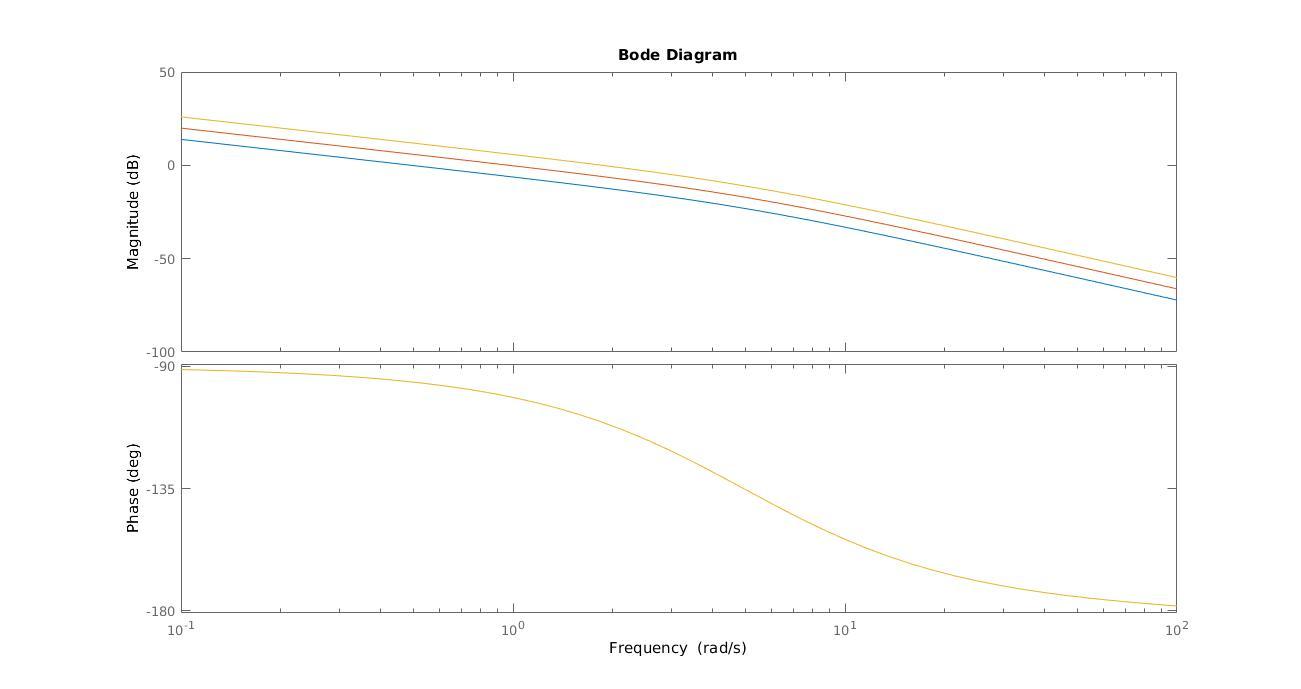
\includegraphics[width=1\textwidth]{figures/G_thetabode.jpg}
	
	
	\caption${G_{\theta}$ bode plot} 
 	\label{fig:gthetabode} 
\end{figure}

\begin{figure} 
\centering
 	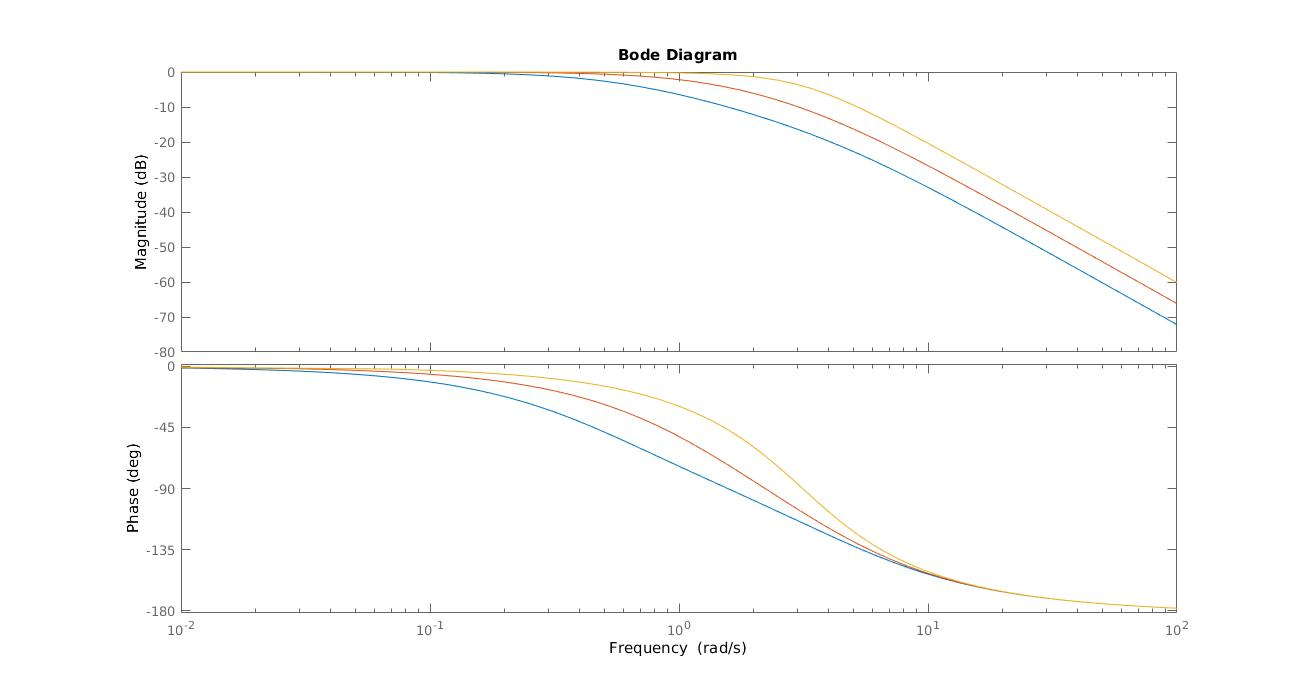
\includegraphics[width=1\textwidth]{figures/Hthetabode.jpg}
	
	
	\caption{$H_{\theta}$ bode plot} 
 	\label{fig:hthetabode} 
\end{figure}

\begin{figure} 
\centering
 	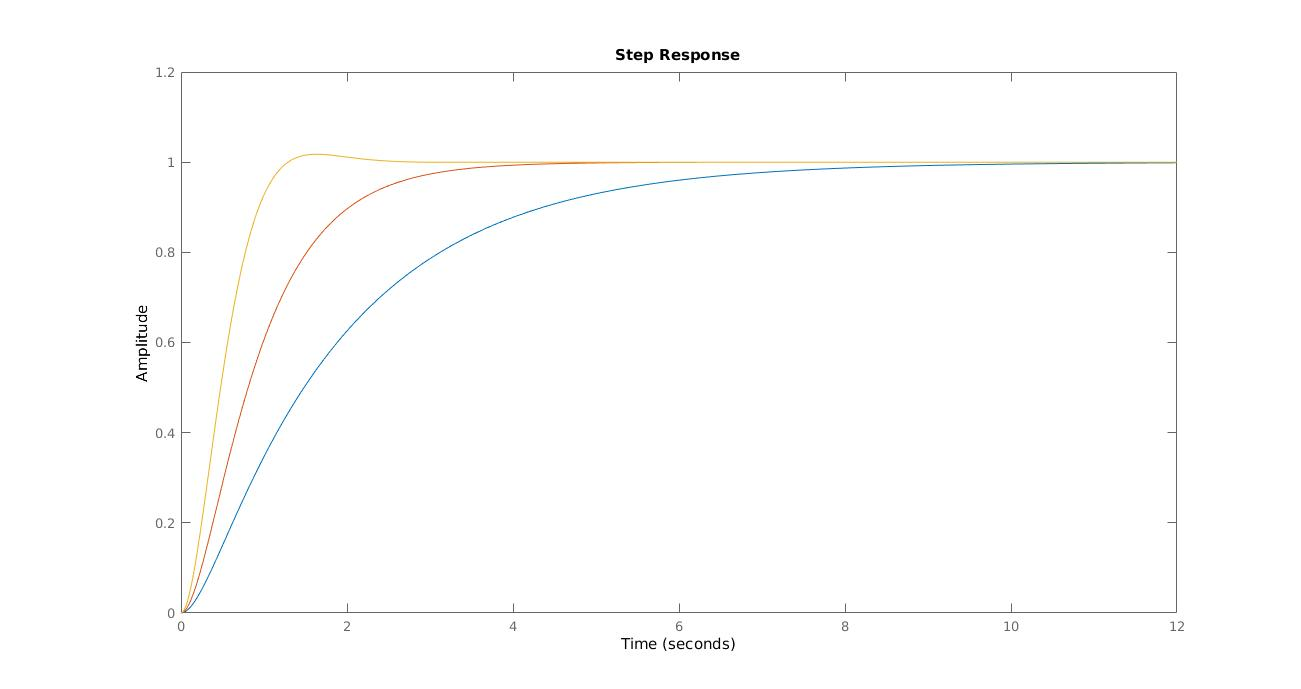
\includegraphics[width=1\textwidth]{figures/thetastep.jpg}
	
	
	\caption{$\Theta$ step response} 
 	\label{fig:thetastep} 
\end{figure}

\section{Kinematic Model Analysis}

A system is said to be controllable if there exists a control law u(.) which can
transfer the state of the system from any initial state x 0 to any final state x f within
a finite amount of time. Otherwise the system is said to be uncontrollable {\color{red} REFERENCE TO sAME BOOK HE HAD}

We will now look more closely the kinematics model and determine if it is controllable or not. The kinematic model is described with the following equations.

\begin{equation} \label{eq74}
\begin{pmatrix} 
 \dot{x} \\ 
 \dot{y} \\
 \dot{\Theta}\\
 \end{pmatrix} 
 =
 \begin{pmatrix}  
 \cos\theta   & 0 \\ 
 \sin\theta & 0 \\
 0 & 1\\ 
 \end{pmatrix}
 \begin{pmatrix} 
 v \\ 
 \omega\\
 \end{pmatrix} 
\end{equation}

Since we have the $\sin\Theta$ and $\cos\Theta$, the system is defined as non-linear.

To determine the controllability of the system we must check the sufficient conditions given by

\begin{equation} \label{eq75}
rank(h1,h2,[h1,h2])
=
rank
\begin{pmatrix} 
 \cos\Theta & 0 & sin\theta\\ 
 \sin\Theta & 0 & -\cos\theta\\
 0 & 1 & 0\\
 \end{pmatrix} 
=
n
=
3
\end{equation}

where

\begin{equation} \label{eq76}
[h1,h2]
=
\frac{\partial h2}{\partial p}h1
-
\frac{\partial h1}{\partial p}h2
\end{equation}

Since we can see that $m$=$n$=3 we can determine that the system is controllable.  This shows us that indeed you can move to any position on the given plain with the robot.

Before we had the kinematic model in the non-linear form. If we linearise the model about an equilibrium point we obtain the following linearised model of the kinematics.

\begin{equation}
\begin{pmatrix}
\dot{x} \\
\dot{y} \\
\dot{\theta}
\end{pmatrix}
=
\begin{pmatrix}
1 & 0 \\
0 & 0 \\
0 & 1 \\
\end{pmatrix}
\begin{pmatrix}
v \\
\omega
\end{pmatrix}
\end{equation}

After the linearisation we can see that the rank of the controllability matrix is less then $n$. From that we can determine that the controllability of the system has been lost after the linearisation, resulting in the requirement for non-linear control.

\section{Cartesian Stabilization}

Cartesian stabilisation control is necessary to ensure that the robot goes to the intended point.In {\color{red}ref to astolfi book} the transformation method of the posture stabilization is explained, of which cartesian stabilization is a subset. Thus we can solve the problem by using non-linear control. 

First we need to transform the kinematic model \ref{eq74} in the terms of the angular and linear displacements.

\begin{equation}
\dot{s}=v\\
\dot{\Theta}=\omega
\end{equation}

Next we define a new state vector $\rho$

\begin{equation}
\rho
=
\begin{pmatrix}
s\\
\Theta
\end{pmatrix}
\end{equation}

Furthermore we will rewrite the state equations as $\dot{\rho}$.
\begin{equation}
\dot{\rho}=
\begin{pmatrix}
v\\
\omega
\end{pmatrix}
\end{equation}
The transformed system will be used in order to make the robot go towards the goal point. Figure \ref{fig:cartesianstab} shows this system.

\begin{figure} 
\centering
 	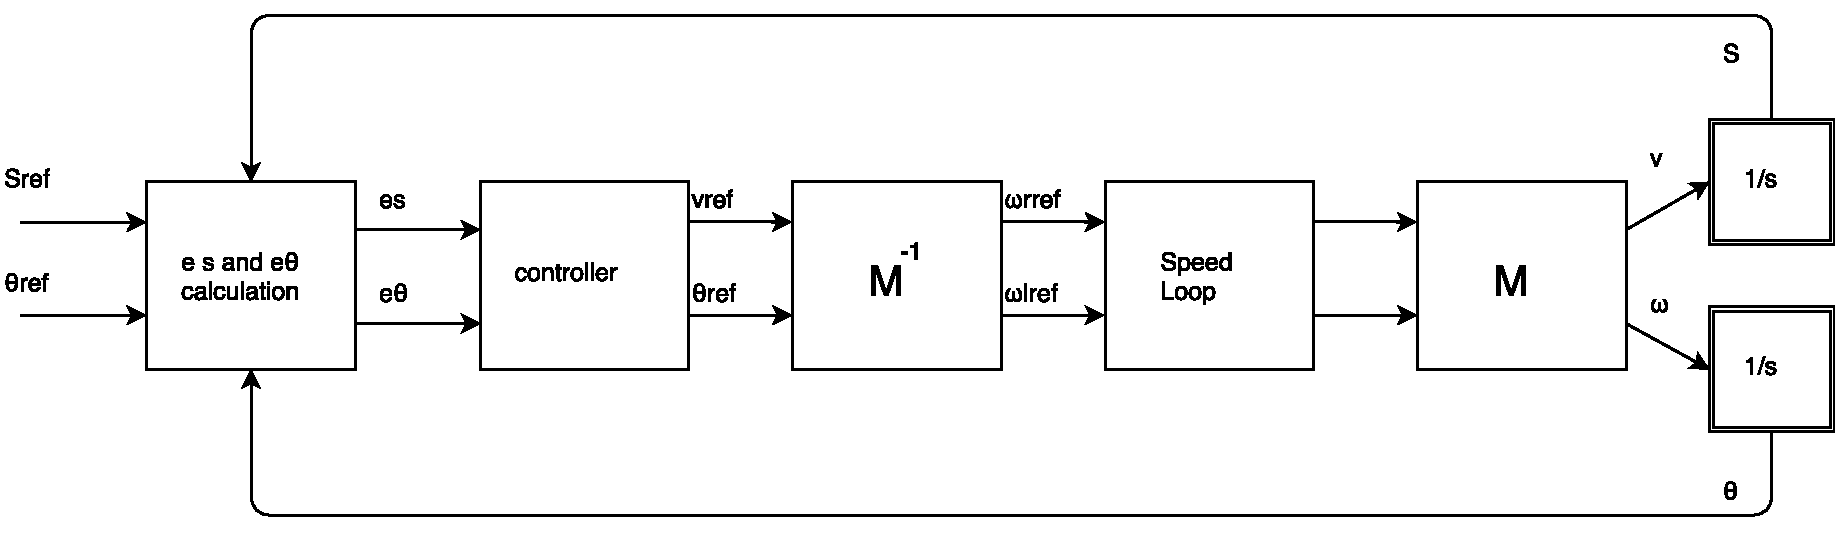
\includegraphics[width=1\textwidth]{figures/cartesianstab.pdf}
	
	
	\caption{Cartesian stabilization} 
 	\label{fig:cartesianstab} 
\end{figure}

As we can see from the figure \ref{fig:cartesianstab} we would neet to get the value of $S_{ref}$. On closer examination we can say that the value of $S_{ref}$ is useless for us and measuring the $S$ is difficult. The problem can be delt with some manipulations as it is explained in{\color{red}Vieira, F.C.; Medeiros, A.A.D.; Alsina P.J.; Araujo A.P. REF THIS}

